\documentclass[12pt, a4paper, oneside]{article}
\usepackage[margin=2cm]{geometry}
\usepackage[utf8]{inputenc}
\usepackage{lipsum}
\usepackage{lastpage}
\usepackage{secdot}
\usepackage{minted}
\usepackage{amsmath}
\usepackage{amssymb}
\usepackage{parskip}  
\usepackage{fancyhdr}
\usepackage{enumerate}
\usepackage[shortlabels]{enumitem}
\usepackage{graphicx}
\usepackage{mathabx}
\graphicspath{ {images/}}

% Definitionen auf neuer Zeile
\setdescription{labelsep=\textwidth}
  
% Define 'variables'
\newcommand{\noteDate}{2017-09-19}
\newcommand{\subjectIdentifier}{BZG1151 DISMAT} 
\newcommand{\subject}{Diskrete Mathematik}

% Set header and footer content
\pagestyle{fancy} 
\fancyhead[L]{Severin Kaderli} 
\fancyhead[C]{\subject{}}
\fancyhead[R]{\noteDate{}}
\fancyfoot[C]{}
\fancyfoot[R]{Seite \thepage{} von \pageref{LastPage}}

% Adjust width of header and footer line
\renewcommand{\headrulewidth}{1pt}
\renewcommand{\footrulewidth}{1pt}

% Move title up and don't show date
\title{\vspace{-1.5cm}\subjectIdentifier{}\\\subject{}}
\author{\vspace{-1.5cm}}
\date{\vspace{-1.5cm}}

\begin{document}
\maketitle
\thispagestyle{fancy}

% Actual content
\section{Modulinformationen}
{\bf Dozentin}: Vidushi Bigler\\
{\bf Kursunterlagen}: https://moodle.bfh.ch/course/view.php?id=15705\\
{\bf Moodle Passwort}: diskMath-17

\newpage
\section{Diskrete Mathematik}
Diskrete Mathematik umfasst verschiedene Teilgebiete der Mathematik, die sich mit mathematischen Operationen über abzählbaren Mengen (endlich und unendlich) beschäftigen. Durch die Entwicklung von Computern wurde die Anwendung der diskreten Mathematik vorangetrieben.

Teilgebiete der diskreten Mathematik umfassen unter anderem:
\begin{itemize}
  \item Logik
  \item Mengenlehre: Relationen, Graphentheorie
  \item Kryptologie
  \item Graphenthorie: Information in Knoten und Kanten darstellen
\end{itemize}

\newpage
\section{Aussagenlogik}
Eine Aussage ist ein sprachliches Gebilde, die entweder wahr oder falsch sein kann. Das Resultat einer Aussage nennt man Wahrheitswert und dieser ist zweiwertig, da er nur zwei Werte (wahr und falsch) annehmen kann.

\newpage
\subsection{8-Damen-Problem}
Auf einem 8 mal 8 Schachbrett sollen 8 Damen platziert werden, ohne dass sie sich gegenseitig angreifen können.

\begin{center}
  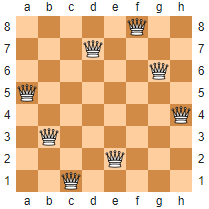
\includegraphics[width=0.5\textwidth]{8queens.png}
\end{center}

Die obige Lösung für das 8-Damen-Problem kann man als Aussage folgendermassen formulieren:

\begin{equation}
  D_{1c} \land D_{2e} \land D_{3b} \land D_{5a} \land D_{7d} \land D_{8f} \land D_{6g} \land D_{4h}
\end{equation}


\subsection{Konjunktion $A \land B$}
AND-Verknüpfung die wahr ist, wenn A und B wahr sind.

\begin{equation}
  \begin{tabular}{| c | c | c |}
    \hline
    $A$ & $B$ & $A \land B$ \\ \hline
    0 & 0 & 0 \\ \hline
    0 & 1 & 0 \\ \hline 
    1 & 0 & 0 \\ \hline
    1 & 1 & 1 \\ \hline
  \end{tabular}
\end{equation}


\subsection{Disjunktion $A \lor B$}
OR-Verknüpfung, die wahr ist, wenn A oder B wahr sind.

\begin{equation}
  \begin{tabular}{| c | c | c |}
    \hline
    $A$ & $B$ & $A \lor B$ \\ \hline
    0 & 0 & 0 \\ \hline
    0 & 1 & 1 \\ \hline
    1 & 0 & 1 \\ \hline
    1 & 1 & 1 \\ \hline
  \end{tabular}
\end{equation}


\subsection{XOR-Verknüpfung $\oplus$}
Verknüpfung, die wahr ist, wenn entweder A oder B wahr sind.

\begin{equation}
  \begin{tabular}{| c | c | c |}
    \hline
    $A$ & $B$ & $A \oplus B$ \\ \hline
    0 & 0 & 0 \\ \hline
    0 & 1 & 1 \\ \hline
    1 & 0 & 1 \\ \hline
    1 & 1 & 0 \\ \hline
  \end{tabular}
\end{equation}


\subsection{Negation $\lnot$}
Die Negation ist wahr, wenn A falsch ist und falsch, wenn A wahr ist.

\begin{equation}
  \begin{tabular}{|c |c |}
    \hline
    $A$ & $\lnot A$ \\ \hline
    0 & 1 \\ \hline
    1 & 0 \\ \hline
  \end{tabular}
\end{equation}


\subsection{Zusammengesetzte Aussagen}
Man kann verschiedene Aussagen zu einer grösseren zusammengesetzten Aussage zusammenschliessen. Eine Zusammengesetze Aussage $P(A_{1}, A_{2}..., A_{N})$ enthält $2^{n}$ Zeilen in der Wahrheitstabelle und kann aus bis zu $(2)^{2^{n}}$ Wahrheitstabellen bestehen.

Auch zu diesen zusammengesetzten Aussagen kann man eine Wahrheitstabelle erstellen. Hier im Beispiel die Aussage $A \land (B \lor A)$.

\begin{equation}
  \begin{tabular}{| c | c | c | c |}
    \hline
    $A$ & $B$ & $B \lor A$ & $A \land (B \lor A)$ \\ \hline
    0 & 0 & 0 & 0 \\ \hline
    0 & 1 & 1 & 0 \\ \hline
    1 & 0 & 1 & 1 \\ \hline
    1 & 1 & 1 & 1 \\ \hline
  \end{tabular}
\end{equation}

\newpage
\subsection{Disjunktive Normalform}
Um die Disjunktive Normalform einer Wahrheitstabelle zu erstellen muss man nur die Zeilen beachten die wahr sind. Die einzelnen Ausdrücke dieser Zeile verbindet man nun durch Konjunktionen und die einzelnen Zeilen dann noch durch Disjunktionen. 

Zur untenstehenden Wahrheitstabelle kann man also folgende Disjunktive Normalform schreiben:

\begin{equation}
  (\lnot A \land B) \lor (A \land \lnot B) \lor (A \land B)
\end{equation}

\begin{equation}
  \begin{tabular}{|c|c|c|}
  \hline
  $A$ & $B$ & $A \lor B$ \\ \hline
  0 & 0 & 0 \\ \hline
  0 & 1 & 1 \\ \hline
  1 & 0 & 1 \\ \hline
  1 & 1 & 1 \\ \hline
  \end{tabular}
\end{equation} 

\subsection{Tautologien und Kontradiktionen}
Eine zusammengesetzte Aussage $P(A, B,...)$, die in der letzten Spalte der Wahrheitstabelle nur wahr ist, wird Tautologie genannt.

Eine zusammengesetzte Aussage $P(A, B,...)$, die in der letzten Spalte der Wahrheitstabelle nur falsh ist, wird Kontradiktion genannt.

\subsection{Logische Äquivalenz}
Zwei zusammengesetzte Aussagen $P(A, B,...)$ und $Q(A, B,...)$ sind logisch äquivalent, wenn sie die gleichen Wahrheitstabellen besitzen. Die logische Äquivalenz kann man folgendermassen schreiben:
\begin{equation} 
  P(A, B,...) \equiv Q(A, B,...)
\end{equation}

\subsection{Implikation}
Eine Aussage in der Form: "Wenn A, dann B.". Solche Aussagen nennt man Implikationen und werden mit der folgenden Schreibweise gekennzeichnet:
\begin{equation}
  A \Rightarrow B 
\end{equation}

Wenn man die Implikation umdreht ist sie nicht logisch äquivalent.
\begin{equation}
  A \Rightarrow B \not\equiv B \Rightarrow A
\end{equation}

Hier die Wahrheitstabelle für die Implikation:
\begin{equation}
  \begin{tabular}{|c|c|c|}
    \hline
    $A$ & $B$ & $A \Rightarrow B$ \\ \hline
    0 & 0 & 1 \\ \hline
    0 & 1 & 1 \\ \hline
    1 & 0 & 0 \\ \hline
    1 & 1 & 1 \\ \hline
  \end{tabular}
\end{equation}

\newpage
\section{Prädikatenlogik}
\subsection{Aussageform}
Eine Aussageform (Prädikat) ist eine Folge von Wörtern mit Leerstellen, die zu einer wahren oder falschen Aussage wird, wenn in jeder Leerstelle ein Eigenname (oder Variable) aus einer vorgegebenen Definitionsmenge eingesetzt wird.

Ein Element $f$ in der Menge $F$ kann man folgendermassen darstellen:

\begin{equation}
  f \in F
\end{equation}

\subsection{Quantoren}
Quantoren sind Operatoren wie die Junktoren. Es gibt die Quantoren für eine Allaussage $\forall$ und für die Existenzprüfung $\exists$. Wenn man betonen will, dass es nur ein Element gibt kann man den Quantor $\exists!$ verwenden.

Beispiel für die Nutzung von Quantoren (P ist die Menge der Primzahlen):
\begin{equation}
  \exists!\ p \in P : (p\ ist\ gerade)
\end{equation}

\newpage
\section{Mengenlehre}
Eine Menge ist eine Sammlung von Elementen die einen Zusammenhang haben. In folgenden Beispielen ist $P$ ein Element bzw. nicht ein Element von der Menge $A$.
 
\begin{equation}
  p \in A
\end{equation}

\begin{equation}
  p \notin A
\end{equation}

und $A = B$ ist genau dann wenn $A = B \equiv \forall x (x \in A \equiv x \in B)$

\subsection{Teilmengen}
Fall jedes Element von A in B vorkommt, ist A eine Teilmenge von B.
\begin{equation}
  A \subset B \Rightarrow \forall x \in U : (x \in A \Rightarrow x \in B)
\end{equation}

\subsection{Vereinigung}
Die Vereinigung der Mengen $A$ und $B$ ist die Menge der Elemente die $A$ oder in $B$ sind. Man schreibt die Vereinigung (Union) folgendermassen.

\begin{equation}
  A \cup B := \{x : x \in A \lor x \in B\}
\end{equation}

\subsection{Durchschnitt}
Der Durchschnitt der Mengen $A$ und $B$ sind die Elemente die in $A$ und $B$ vorkommen. Man schreibt den Durchschnitt folgendermassen.

\begin{equation}
  A \cap B := \{x : x \in A \land x \in B\}
\end{equation}

\subsection{Komplement}
Das Komplement der Menge, ist die Menge der Elemente von $U$, die nicht zu $A$ gehören.

\begin{equation}
  A^\complement := \{x : x \in U \land x \notin A\}
\end{equation}

\subsection{Differenz}
Die Differenz der Mengen $A$ und $B$, ist die Menge der Elemente von $A$, die nicht in $B$ vorkommen.

\begin{equation}
  A \setminus B := \{x : x \in A \land x \notin B\}
\end{equation}

\subsection{Mengensystem}
Eine Menge von Mengen heisst Mengensystem. Das System aller Teilmengen einer Menge $S$ heisst Potenzmenge und wird mit $P(S)$ bezeichnet. Falls man eine Menge $S = \{1, 2\}$ hat dann ist die Potenzmenge von $S$:

\begin{equation}
  P(S) = \{\varnothing, \{1\}, \{2\}, \{1, 2\}\}
\end{equation}

Eine Partition von der Menge S, ist die Aufteilung von S in nicht-leere Teilmengen, welche sich nicht überlappen. Beispielweise hat man eine Menge $A = \{1, 2, 3, 4, 5, 6, 7\}$. Eine mögliche Partition dafür wäre:

\begin{equation}
  \{\{1, 2\}, \{3, 4, 5, 6\}, \{7\}\}
\end{equation}


\subsection{Geordnete Paare}
Bei normalen Mengen spielt die Reihenfolge der Elemente keine Rolle.

\begin{equation}
  \{a, b\} = \{b, a\}
\end{equation}

Bei einem Geordnetem Paar ist die Reihenfolge aber wichtig. Ein geordnetes Paar schreibt man mit der folgenden Schreibweise:
\begin{equation}
  (a, b) \neq (b, a)
\end{equation}


\subsection{Kartesisches Produkt}
Man hat zwei Mengen $A$ und $B$. Die Menge aller geordneter Paare mit $x \in A$ und $y \in B$ nennt man kartesisches Produkt und wird mit $A \times B$ bezeichnet.
\begin{equation}
  A \times B = \{(x, y) : x \in A \land y \in B\}
\end{equation}

$\rightarrow$ Siehe Beispiel 38 und 39.

\subsection{Endliche Mengen}
Eine Menge heisst endlich, falls sie genau $m$ verschiedene Elemente enthält, wo $m$ eine natürliche Zahl ist. Ansonsten ist die Menge unendlich.

Die leere Menge $\varnothing$ und die Menge der Buchstaben des Alphabetes sind endliche Mengen, während die Menge der positiven ganzen Zahlen $\{1, 2, 3, 4, 5,\dots\}$ unendlich ist.

%%%%%%%%
%
% Gesetze
%
%%%%%%%%
\newpage
\subsection{Gesetze}
\subsubsection{Satz 6}
$A$, $B$ und $C$ sind beliebige Mengen und $\varnothing$ ist die Leere Menge.
\begin{enumerate}[(i)]
  \item $\forall A : (\varnothing \subset A \land A \subset A) $
  \item $\forall A, B, C : (A \subset B \land B \subset C) \Longrightarrow (A \subset C)$
  \item $\forall A, B : (A = B \Longleftrightarrow ((A \subset B) \land (B \subset A)))$
  
\end{enumerate}

\newpage 
\section{Übungsbeispiele aus Skript}
\subsection{Beispiel 8}
\begin{equation}
  (A \land B \land C) \lor (A \land B \land \lnot C) \lor (A \land \lnot B \land \lnot C) \lor (\lnot A \land \lnot B \land C)
\end{equation}

\subsection{Beispiel 9}
  Diese Aussage lässt sich vereinfacht als $C \lor \lnot C$ darstellen. Es handelt sich also um eine Tautologie und alle Zeilen der Wahrheitstabelle sind wahr.
 


\subsection{Beispiel 16}
\begin{equation}
  \begin{tabular}{|c|c|c|c|}
    \hline
    $A$ & $B$ & $\lnot A$ & $\lnot A \lor B$ \\ \hline
    0 & 0 & 1 & 0 \\ \hline
    0 & 1 & 1 & 1 \\ \hline
    1 & 0 & 0 & 0 \\ \hline
    1 & 1 & 0 & 0 \\ \hline
  \end{tabular}
\end{equation}

\subsection{Beispiel 27}
$A = B$ \\
$C$ \\
$D = E$ \\
$F = G$

\subsection{Beispiel 28}
Die Lösung ergibt die Leere Menge, da das Resultat in der Menge der komplexen Zahlen ist.

\begin{equation}
  x = \{\}
\end{equation}

Die eigentliche Lösung im komplexen Zahlenraum wäre:
\begin{equation}
  x = \{+i, -i\}
\end{equation}

\subsection{Beispiel 29}
\begin{enumerate}[a)]
  \item wahr
  \item wahr
  \item falsch
\end{enumerate}

\subsection{Beispiel 30}
\begin{enumerate}
  \item $\{1, 2, 3, 4, 5, 6, 7, 8\}$
  \item $\{\gamma, \delta\}$
  \item $\{\}$
\end{enumerate}

\subsection{Beispiel 31}
 
\subsection{Beispiel 33}

\subsection{Beispiel 34}

\subsection{Beispiel 35} 
\begin{enumerate}[$\bullet$]
  \item $P(A) = \{\varnothing\}$
  \item $P(B) = \{\varnothing,\{a\} \}$
  \item $P(C) = \{\varnothing, \{a\}, \{b\}, \{a, b\}\}$
\end{enumerate}

\subsection{Beispiel 36}
Eine Menge mit $n$ Elementen besitzt $2^{n}$ Teilmengen.

\subsection{Beispiel 37}
\begin{enumerate}[(a)]
  \item falsch (Leere Menge darf kein Teil sein)
  \item falsch (4 überlappt sich)
  \item falsch (Die 1 fehlt)
  \item wahr
\end{enumerate}

\subsection{Beispiel 38}
\begin{equation}
  A \times B = \{(1, a), (1, b), (1, c), (2, a), (2, b), (2, c)\}
\end{equation}

\begin{equation}
  B \times A = \{(a, 1), (a, 2), (b, 1), (b, 2), (c, 1), (c, 2)\}
\end{equation}

\begin{equation}
  A^{2} = A \times A = \{(1, 1), (1, 2), (2, 1), (2, 2)\}
\end{equation}

\subsection{Beispiel 39}
Anzahl der Elemente von $A$ mal die Anzahl der Elemente von $B$ ergibt die Anzahl der Elemente von $A \times B$.


\section{Übungsserien}
\subsection{Serie 3}
\subsubsection{Aufgabe 1}
\begin{enumerate}[(a)]
  \item A = \{4, 5, 6, 7, 8, 9, 10, 11\}
  \item B = \{2, 4, 6, 8, 10, 12, 14\}
  \item C = \{\}
\end{enumerate}

\subsubsection{Aufgabe 2}
\begin{enumerate}[(a)]
  \item \{1, 2, 3, 4, 5, 6, 7\}
  \item \{4, 5\}
  \item \{5, 7, 9\}
  \item \{1, 2, 3, 4, 5, 6, 7, 8, 9\}
  \item \{6, 7, 8, 9\}
  \item \{2, 4, 6, 8\}
  \item \{1, 2, 3\}
  \item \{6, 7\}
  \item \{1, 3\}
  \item \{5, 6, 8\}
\end{enumerate}

\subsubsection{Aufgabe 3}
\begin{enumerate}[(a)]
  \item wahr
  \item wahr
  \item wahr
  \item falsch
  \item wahr
  \item falsch
  \item wahr
  \item falsch
\end{enumerate}

\subsubsection{Aufgabe 4} 
\begin{enumerate}[(a)]
  \item 5
  \item Siehe Bild unten
  \item 38
\end{enumerate}

\subsubsection{Aufgabe 5}
\begin{equation}
  \{x : x \in \mathbb{N} : \}
\end{equation}

\subsubsection{Aufgabe 6}
Kleinkinder können keine Krokodile bezwingen.
 
\end{document}
